\section{Introduction}
Breast cancer is one of the most common cancer along with lung and bronchus cancer, prostate cancer, colon cancer, and pancreatic cancer among others\cite{nci2017}. Representing 15\% of all new cancer cases in the United States alone\cite{surveillance}, it is a topic of research with great value.\\
\indent	The utilization of data science and machine learning approaches in medical fields proves to be prolific as such approaches may be considered of great assistance in the decision making process of medical practitioners. With an unfortunate increasing trend of breast cancer cases\cite{surveillance}, comes also a big deal of data which is of significant use in furthering clinical and medical research, and much more to the application of data science and machine learning in the aforementioned domain.\\
\indent	Prior studies have seen the importance of the same research topic\cite{salama2012breast, zafiropoulos2006support}, where they proposed the use of machine learning (ML) algorithms for the classification of breast cancer using the Wisconsin Diagnostic Breast Cancer (WDBC) dataset\cite{wolberg1992breast}, and eventually had significant results.\\
\indent	This paper presents yet another study on the said topic, but with the introduction of our recently-proposed GRU-SVM model\cite{agarap2017neural}. The said ML algorithm combines a type of recurrent neural network (RNN), the gated recurrent unit (GRU)\cite{Cho} with the support vector machine (SVM)\cite{Cortes}. Along with the GRU-SVM model, a number of ML algorithms is presented in Section \ref{ml-algorithms}, which were all applied on breast cancer classification with the aid of WDBC\cite{wolberg1992breast}.

\section{Methodology}

\subsection{Machine Intelligence Library}
Google TensorFlow\cite{tensorflow2015-whitepaper} was used to implement the machine learning algorithms in this study, with the aid of other scientific computing libraries: matplotlib\cite{Hunter:2007}, numpy\cite{walt2011numpy}, and scikit-learn\cite{scikit-learn}. 

\subsection{The Dataset}
The Wisconsin Diagnostic Breast Cancer (WDBC) dataset\cite{wolberg1992breast} was used to implement the machine learning algorithms (in Section \ref{ml-algorithms}) for breast cancer diagnosis. According to \cite{wolberg1992breast}, the dataset consists of features which were computed from a digitized image of a fine needle aspirate (FNA) of a breast mass. The said features describe the characteristics of the cell nuclei found in the image\cite{wolberg1992breast}.
\begin{figure}[!htb]
\minipage{0.45\textwidth}
\centering
	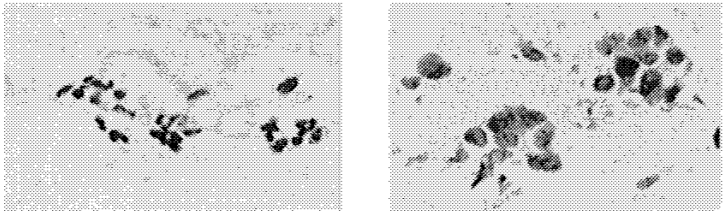
\includegraphics[width=\linewidth]{fna_image.png}
	\caption{Image from \cite{wolberg1992breast} as cited by \cite{zafiropoulos2006support}. Digitized images of FNA: (a) Benign, (b) Malignant.}
	\label{training-accuracy}
\endminipage\hfill
\end{figure}

\indent	There are 569 data points in the dataset: 212 -- Malignant, 357 -- Benign. Accordingly, the dataset features are as follows: (1) radius, (2) texture, (3) perimeter, (4) area, (5) smoothness, (6) compactness, (7) concavity, (8) concave points, (9) symmetry, and (10) fractal dimension.\\
\indent	With each feature having three information\cite{wolberg1992breast}: (1) mean, (2) standard error, and (3) ``worst'' or largest (mean of the three largest values) computed. Thus, having a total of 30 dataset features.

\subsection{Dataset Preprocessing}

To avoid inappropriate assignment of relevance, the dataset was standardized using Eq. \ref{student-t-stat}.

\begin{equation}\label{student-t-stat}
z=\dfrac{X - \mu}{\sigma}
\end{equation}

where $X$ is the feature to be standardized, $\mu$ is the mean value of the feature, and $\sigma$ is the standard deviation of the feature. The standardization was implemented using \texttt{StandardScaler().fit\_transform()} of \texttt{scikit-learn}\cite{scikit-learn}.

\subsection{Machine Learning (ML) Algorithms}\label{ml-algorithms}

This section presents the machine learning (ML) algorithms used in the study. The Stochastic Gradient Descent (SGD) learning algorithm was used for all the ML algorithms presented in this section except for GRU-SVM, Nearest Neighbor search, and Support Vector Machine. The code implementations may be found online at https://github.com/AFAgarap/wisconsin-breast-cancer.

\subsubsection{GRU-SVM}
We proposed a neural network architecture\cite{agarap2017neural} combining the gated recurrent unit (GRU) recurrent neural network (RNN) and the support vector machine (SVM), for the purpose of binary classification.
\begin{equation}\label{z-gate}
z	=	\sigma(\vec{W}_{z} \cdot [h_{t - 1}, x_{t}])
\end{equation}
\begin{equation}\label{r-gate}
r	=	\sigma(\vec{W}_{r} \cdot [h_{t - 1}, x_{t}])
\end{equation}
\begin{equation}\label{candidate-value}
\tilde{h}_{t}	=	tanh(\vec{W} \cdot [r_{t} * h_{t - 1}, x_{t}])
\end{equation}
\begin{equation}\label{new-value}
h_{t}	=	(1 - z_{t}) * h_{t - 1} + z_{t} * \tilde{h}_{t}
\end{equation}

where $z$ and $r$ are the \textit{update gate} and \textit{reset gate} of a GRU-RNN respectively, $\tilde{h}_{t}$ is the candidate value, and $h_{t}$ is the new RNN cell state value\cite{Cho}. In turn, the $h_{t}$ is used as the input in the L2-SVM classifier (see Eq. \ref{l2-svm} in Section \ref{svm}) of the network instead of the conventional Softmax classifier. Then, the Adam\cite{Kingma} algorithm was used to learn the parameters $\vec{W}$ to minimize the loss $L$ of the model. The same learning algorithm was used for the implementation of SVM (Section \ref{svm}) in this study.

\subsubsection{Linear Regression}\label{linear-regression}
Despite an algorithm for regression problem, linear regression (see Eq. \ref{linear-regression-equation}) was used as a classifier for this study. This was done by applying a threshold for the output of Eq. \ref{linear-regression-equation}, i.e. subjecting the value of the regressand to Eq. \ref{threshold}.
\begin{align}\label{linear-regression-equation}
h_{\theta}(x)	&= \sum_{i=0}^{n} \theta_{i} \cdot \vec{x}_{i}
\end{align}
\begin{align}\label{threshold}
f\big(h_{\theta}(x)\big)	=	\begin{cases}
									1	&	h_{\theta}(x) \geq 0.5	\\
									0	&	h_{\theta}(x) < 0.5
								\end{cases}
\end{align}

To measure the loss of the model, the mean squared error (MSE) was used (see Eq. \ref{mse}). 
\begin{align}\label{mse}
L(y, \theta, x)	&=	\dfrac{1}{N} \sum_{i = 0}^{N} \big((\vec{\theta_{i}} \cdot \vec{x}_{i}) - y_{i} \big)^{2}
\end{align}

where $y$ represents the actual class, and $(\vec{\theta} \cdot \vec{x})$ represents the predicted class. This loss is minimized through the use of SGD algorithm, which learns the parameters $\theta$ of Eq. \ref{linear-regression-equation}. The same method of loss minimization could be said for MLP and Softmax Regression.

\subsubsection{Multilayer Perceptron}
The perceptron model was developed by Rosenblatt (1958)\cite{rosenblatt1958perceptron} based on the neuron model by McCulloch \& Pitts (1943)\cite{mcculloch1943logical}. The multilayer perceptron (MLP)\cite{bishop1995neural} consists of hidden layers (composed by a number of perceptrons) that enables the approximation of any functions, that is, through activation functions such as $tanh$ or \textit{sigmoid} $\sigma$.
\begin{align}
h_{\theta}(x)	&=	\sum_{i = 0}^{n} \vec{\theta}_{i} \vec{x}_{i}
\end{align}
\begin{align}\label{relu}
f\big(h_{\theta}(x)\big)	&= \vec{h_{\theta}(x)}^{+} = max(0, \vec{h_{\theta}(x)})
\end{align}

For this study, the activation function used for MLP was ReLu\cite{hahnloser2000digital} (see Eq. \ref{relu}), while there were three hidden layers that each consists of 500 nodes (500-500-500 architecture). As for the loss, it was computed using the cross entropy function (see Eq. \ref{cross-entropy}).

\subsubsection{Nearest Neighbor}
This is a form of an optimization problem that seeks to find the closest point $p_{i} \in \vec{p}$ to a query point $q_{i} \in \vec{q}$. In this study, both the L1 (Manhattan, Eq. \ref{taxicab-norm}) and L2 (Euclidean, Eq. \ref{euclidean-norm}) norm were used to measure the distance between $\vec{p}$ and $\vec{q}$.
\begin{equation}\label{taxicab-norm}
        \begin{gathered}
                \|\vec{p} - \vec{q}\|_{1} = \sum_{i=1}^{n} |p_{i} - q_{i}|
        \end{gathered}
\end{equation}
\begin{equation}\label{euclidean-norm}
        \begin{gathered}
                \|\vec{p} - \vec{q}\|_{2} = \sqrt{\sum_{i=1}^{n} (p_{i} - q_{i})^{2}}
        \end{gathered}
\end{equation}

The code implementation was based on the work of Damien (2017)\cite{aymericdamien} in GitHub. A learning algorithm such as SGD and Adam\cite{Kingma} is not applicable to Nearest Neighbor search, as it is practically a geometric approach for classification.

\subsubsection{Softmax Regression}
This is a classification model generalizing logistic regression to multinomial problems. But unlike linear regression (Section \ref{linear-regression}) that produces raw scores for the classes, softmax regression produces a probability distribution for the classes. This is accomplished using the Softmax function (see Eq. \ref{softmax}).
\begin{align}\label{softmax}
P(\vec{y}_{i}\ |\ \vec{x})	&= \dfrac{e^{h_{\theta}(x)_{i}}}{\sum_{i=0}^{n} e^{h_{\theta}(x)_{i}}}
\end{align}

\begin{align}\label{cross-entropy}
L(y, \theta, x)	&=	-\sum_{i = 0}^{n} y_{i} \cdot log\big(h_{\theta}(x)_{i}\big)
\end{align}

The loss is measured by using the cross entropy function (see Eq. \ref{cross-entropy}), where $y$ represents the actual class, and $h_{\theta}(x)$ represents the predicted class.

\subsubsection{Support Vector Machine}\label{svm}
Developed by Vapnik\cite{Cortes}, the support vector machine (SVM) was primarily intended for binary classification. Its main objective is to determine the optimal hyperplane $f(w, x) = \vec{w} \cdot \vec{x} + b$ separating two classes in a given dataset having input features $\vec{x} \in \mathbb{R}^{p}$, and labels $\vec{y} \in \{-1, +1\}$.

SVM learns by solving the following constrained optimization problem:
\begin{equation} \label{constrained-l1}
min \dfrac{1}{2}\vec{w}^{T}\vec{w} + C \sum_{i = 1}^{p} \xi_i
\end{equation}
\begin{align}
s.t\ y_{i}'(\vec{w} \cdot \vec{x} + b) \geq 1 - \xi_i\\
\xi_i \geq 0, i = 1, ..., p
\end{align}

where $\vec{w}^{T} \vec{w}$ is the Manhattan norm, $\xi$ is a cost function, and $C$ is the penalty parameter (may be an arbitrary value or a selected value using hyper-parameter tuning). The corresponding unconstrained optimization problem (Eq. \ref{constrained-l1}) is the following:
\begin{equation} \label{l1-svm}
min \dfrac{1}{2}\vec{w}^{T}\vec{w} + C \sum_{i = 1}^{p} max\big(0, 1 - y_{i}'(\vec{w}^{T}\vec{x}_{i}+b)\big)
\end{equation}

\indent where $\vec{w}^T\vec{x}_{i} + b_{i}$ is the predictor function. The objective of Eq. \ref{l1-svm} is known as the primal form problem of L1-SVM, with the standard hinge loss. The problem with L1-SVM is the fact that it is not differentiable\cite{Tang}, as opposed to its variation, the L2-SVM:
\begin{equation}\label{l2-svm}
min \dfrac{1}{2}\|\vec{w}\|_{2}^{2} + C \sum_{i = 1}^{p} max\big(0, 1 - y_{i}'(\vec{w}^{T}\vec{x}_{i}+b)\big)^{2}
\end{equation}

The L2-SVM is differentiable and provides more stable results than its L1 counterpart\cite{Tang}. However, for this study, the regularizer used was Eq. \ref{regularizer}. Along with the said change, the hinge loss used was Eq. \ref{hinge-loss}.
\begin{align}\label{regularizer}
R(w)	&=	\dfrac{1}{N} \sum_{i}^{N} w_{i}^{2}
\end{align}
\begin{align}\label{hinge-loss}
L	&= \dfrac{1}{p} \sum_{i = 1}^{p} max\big(0, 1 - y_{i}'(\vec{w}^{T}\vec{x}_{i}+b)\big)^{2}
\end{align}

Eq. \ref{regularizer} is the L2-Norm, but with an amendment with its $\lambda$ parameter of $\frac{1}{N}$. As for Eq. \ref{hinge-loss}, its mean value is computed with the introduction of $\frac{1}{p}$, then it is multiplied by the penalty parameter $C$. Essentially still Eq. \ref{l2-svm}, but with different parameters: $R(w) + C \cdot L$.

\subsection{Data Analysis}
There were two phases of experiment for this study: (1) training phase, and (2) test phase. All the ML algorithms described in Section \ref{ml-algorithms} were trained and tested on WDBC. The dataset was partitioned by 70\% (training phase) / 30\% (testing phase).\\
\indent	The parameters considered in the experiments were the following: (1) Test Accuracy, (2) Epochs, (3) Number of data points, (4) False Positive Rate (FPR, Eq. \ref{FPR}), (5) False Negative Rate (FNR, Eq. \ref{FNR}), (6) True Positive Rate (TPR, Eq. \ref{TPR}), and (7) True Negative Rate (TNR, Eq. \ref{TNR}).

\begin{align}\label{TPR}
TPR	&=	\dfrac{True\ Positive}{True\ Positive + False\ Negative}
\end{align}
\begin{align}\label{TNR}
TNR	&=	\dfrac{True\ Negative}{True\ Negative + False\ Positive}
\end{align}
\begin{align}\label{FPR}
FPR	&=	1 - TNR
\end{align}
\begin{align}\label{FNR}
FNR	&=	1 - TPR
\end{align}

\section{Results and Discussion}
All experiments in this study were conducted on a laptop computer with Intel Core(TM) i5-6300HQ CPU @ 2.30GHz x 4, 16GB of DDR3 RAM, and NVIDIA GeForce GTX 960M 4GB DDR5 GPU.
\begin{table*}
\centering
\caption{Hyper-parameters used for the ML algorithms.}
		\begin{tabular}{ccccccc}
		\toprule
		Hyper-parameters & GRU-SVM & Linear Regression & MLP & Nearest Neighbor & Softmax Regression & SVM \\
		\midrule
		Batch Size & 128 & 128 & 128 & N/A & 128 & 128 \\
		Cell Size & 128 & 128 & 128 & N/A & 128 & 128 \\
		Dropout Rate & 0.5 & N/A & None & N/A & N/A & N/A\\
		Epochs & 3000 & 3000 & 3000 & 1 & 3000 & 3000\\
		Learning Rate & 1e-3 & 1e-3 & 1e-2 & N/A & 1e-3 & 1e-3\\
		Norm & L2 & N/A & N/A & L1, L2 & N/A & L2\\
		SVM C & 5 & N/A & N/A & N/A & N/A & 5\\
		\bottomrule
		\end{tabular}\\
		\label{table: hyperparameters}
\end{table*}
\begin{table*}
\centering
\caption{Summary of experiment results on the ML algorithms.}
		\begin{tabular}{cccccccc}
		\toprule
		Parameter & GRU-SVM & Linear Regression & MLP & L1-NN & L2-NN & Softmax Regression & SVM \\
		\midrule
		Accuracy & 93.75\% & 96.09375\% & 99.038449585420729\% & 93.567252\% & 94.736844\% & 97.65625\% & 96.09375\% \\
		Data points  & 384000 & 384000 & 512896 & 171 & 171 & 384000 & 384000 \\
		Epochs & 3000 & 3000 & 3000 & 1 & 1 & 3000 & 3000\\
		FPR & 16.666667\% & 10.204082\% & 1.267042\% & 6.25\% & 9.375\% & 5.769231\% & 6.382979\% \\
		FNR & 0 & 0 & 0.786157\% & 6.542056\% & 2.803738\%& 0 & 2.469136\% \\
		TPR & 100\% & 100\% & 99.213843\% & 93.457944\% & 97.196262\% & 100\% & 97.530864\% \\
		TNR & 83.333333\% & 89.795918\% & 98.732958\% & 93.75\% & 90.625\% & 94.230769\% & 93.617021\% \\
		\bottomrule
		\end{tabular}\\
		\label{table: summary-results}
\end{table*}

\indent	Table \ref{table: hyperparameters} shows the manually-assigned hyper-parameters used for the ML algorithms. The hyper-parameters of a ML algorithm affects its performance in training, speed, and generalization capability. In this study, the hyper-parameters set were not obtained through hyper-parameter optimization / tuning, but they were set by hand. To determine the most optimal hyper-parameters, cross validation (CV) techniques such as $k$-fold cross validation must be used\cite{bengio2015deep}. Unfortunately, this study was limited to the conventional dataset partitioning of 70/30, training dataset and testing dataset respectively. \\
\indent	Table \ref{table: summary-results} summarizes the experiment results. In addition to the reported results, the results from the studies by \cite{salama2012breast} and \cite{zafiropoulos2006support} are put into comparison. First, \cite{salama2012breast} implemented five ML algorithms for classification on WDBC. Namely, (1) Naive Bayes (NB), (2) MLP, (3) SVM, (4) K-Nearest Neighbor (KNN), and (5) Decision Tree J48\cite{quinlan1993c4}. The single classifier algorithms they used were implemented using WEKA\cite{witten2016data}, and their hyper-parameters and architecture (for MLP) were not specified. Their results have shown the following test accuracies: (1) NB had 92.9701\%, (2) MLP had 96.6608\%, (3) SVM had 97.71533\%, (4) KNN had 95.9575\%, and (5) Decision Tree J48 had 93.1459\%. Then, \cite{zafiropoulos2006support} implemented a SVM with Gaussian Radial Basis Function (RBF) as its kernel for classification on WDBC. Their experiment revealed that the said SVM had its highest test accuracy of 89.28\% with its free parameter $\sigma = 0.6$ in Eq. \ref{gaussian-rbf}.
\begin{align}\label{gaussian-rbf}
	K(x, x')	&=	exp\bigg(-\dfrac{\|x - x'\|^{2}}{2\sigma^{2}}\bigg)
\end{align}
\indent	Looking at Table \ref{table: summary-results}, the ML algorithms used in this study may be considered on par with the findings of \cite{salama2012breast} and \cite{zafiropoulos2006support}. With MLP of $500-500-500$ architecture, and its hyper-parameters specified in Table \ref{table: hyperparameters}, it reached a test accuracy of $\approx$99.04\%, comparable to \cite{salama2012breast}. With a test accuracy of $\approx$96.09\%, the L2-SVM lies in the between the findings of \cite{salama2012breast}(WEKA\cite{witten2016data} SVM, 97.71533\%) and \cite{zafiropoulos2006support}(Gaussian RBF, 89.28\%). Meanwhile, the L2-NN is not far from the KNN in \cite{salama2012breast}, with a test accuracy of $\approx$94.74\%. Keeping in mind that the KNN is a generalization of NN that seeks to find $K$ nearest points, while NN seeks to find the closest point $p_{i} \in \vec{p}$ to $q_{i} \in \vec{q}$.\\
\begin{figure}[!htb]
\minipage{0.5\textwidth}\centering
	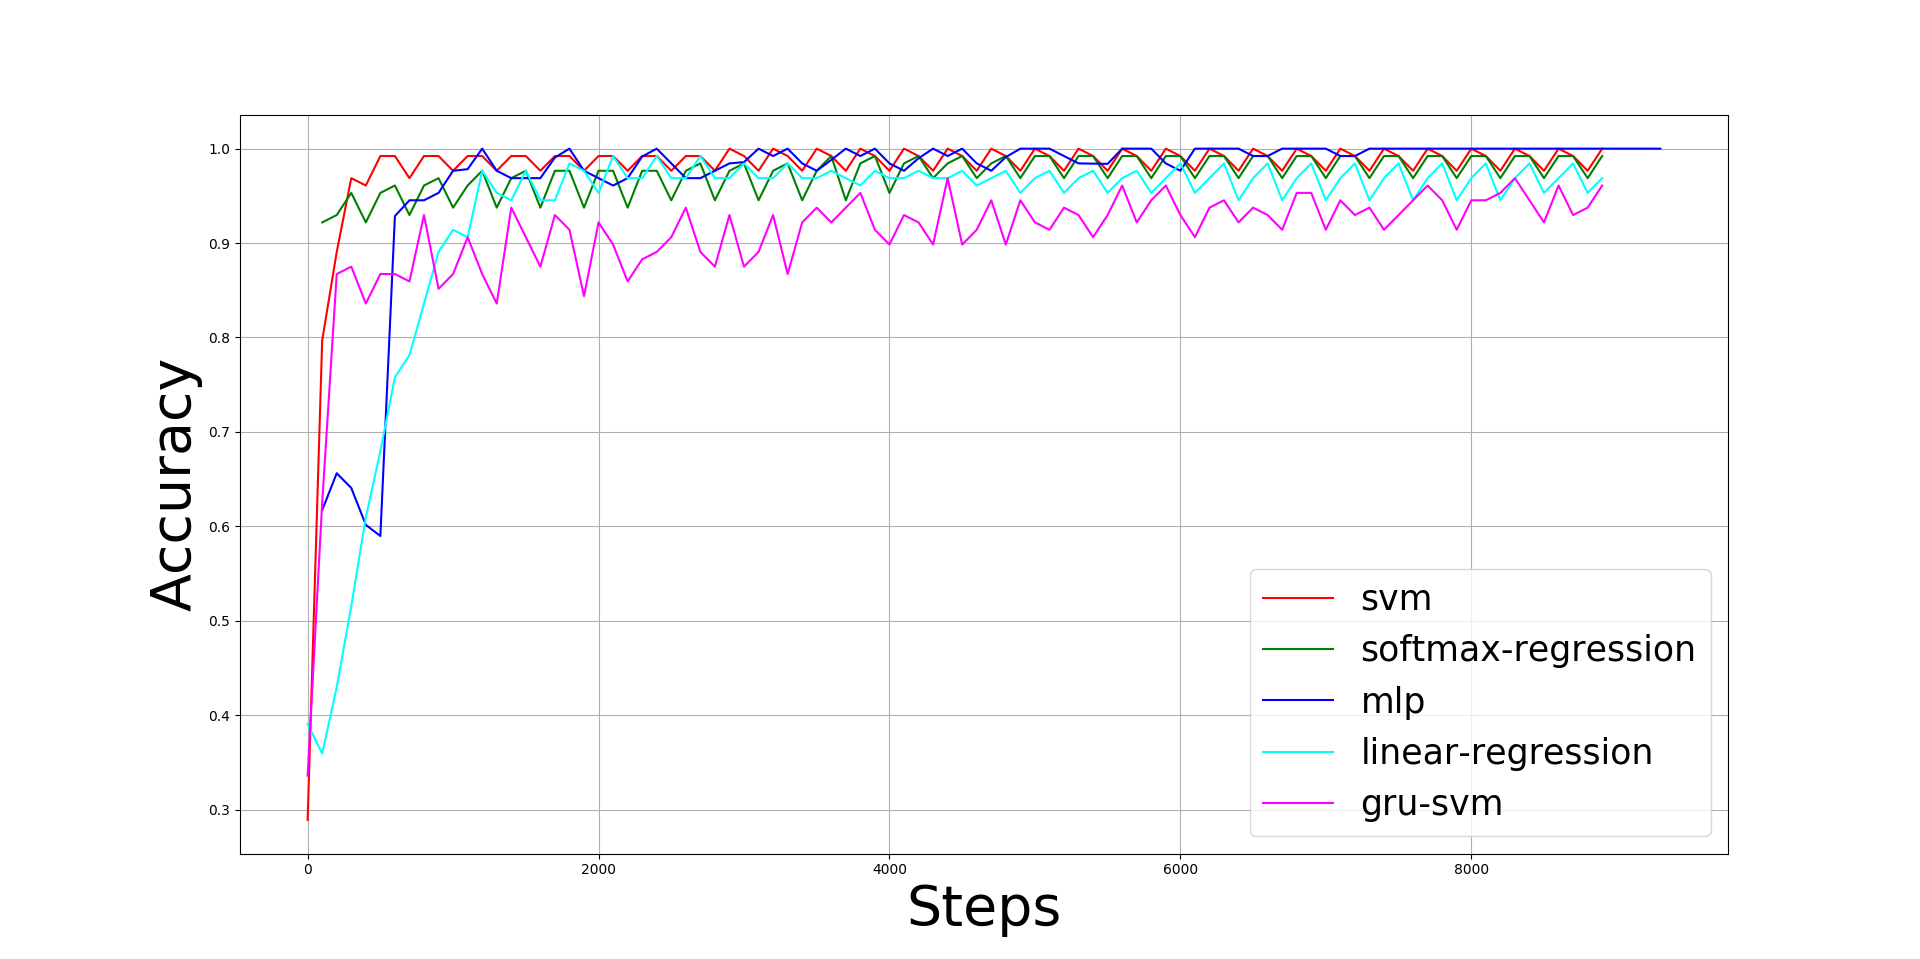
\includegraphics[width=\linewidth]{training_accuracy.png}
	\caption{Plotted using \texttt{matplotlib}\cite{Hunter:2007}. Training accuracy of the ML algorithms on breast cancer detection using WDBC.}
	\label{training-accuracy}
\endminipage\hfill
\end{figure}
\begin{figure}[!htb]
\minipage{0.5\textwidth}\centering
	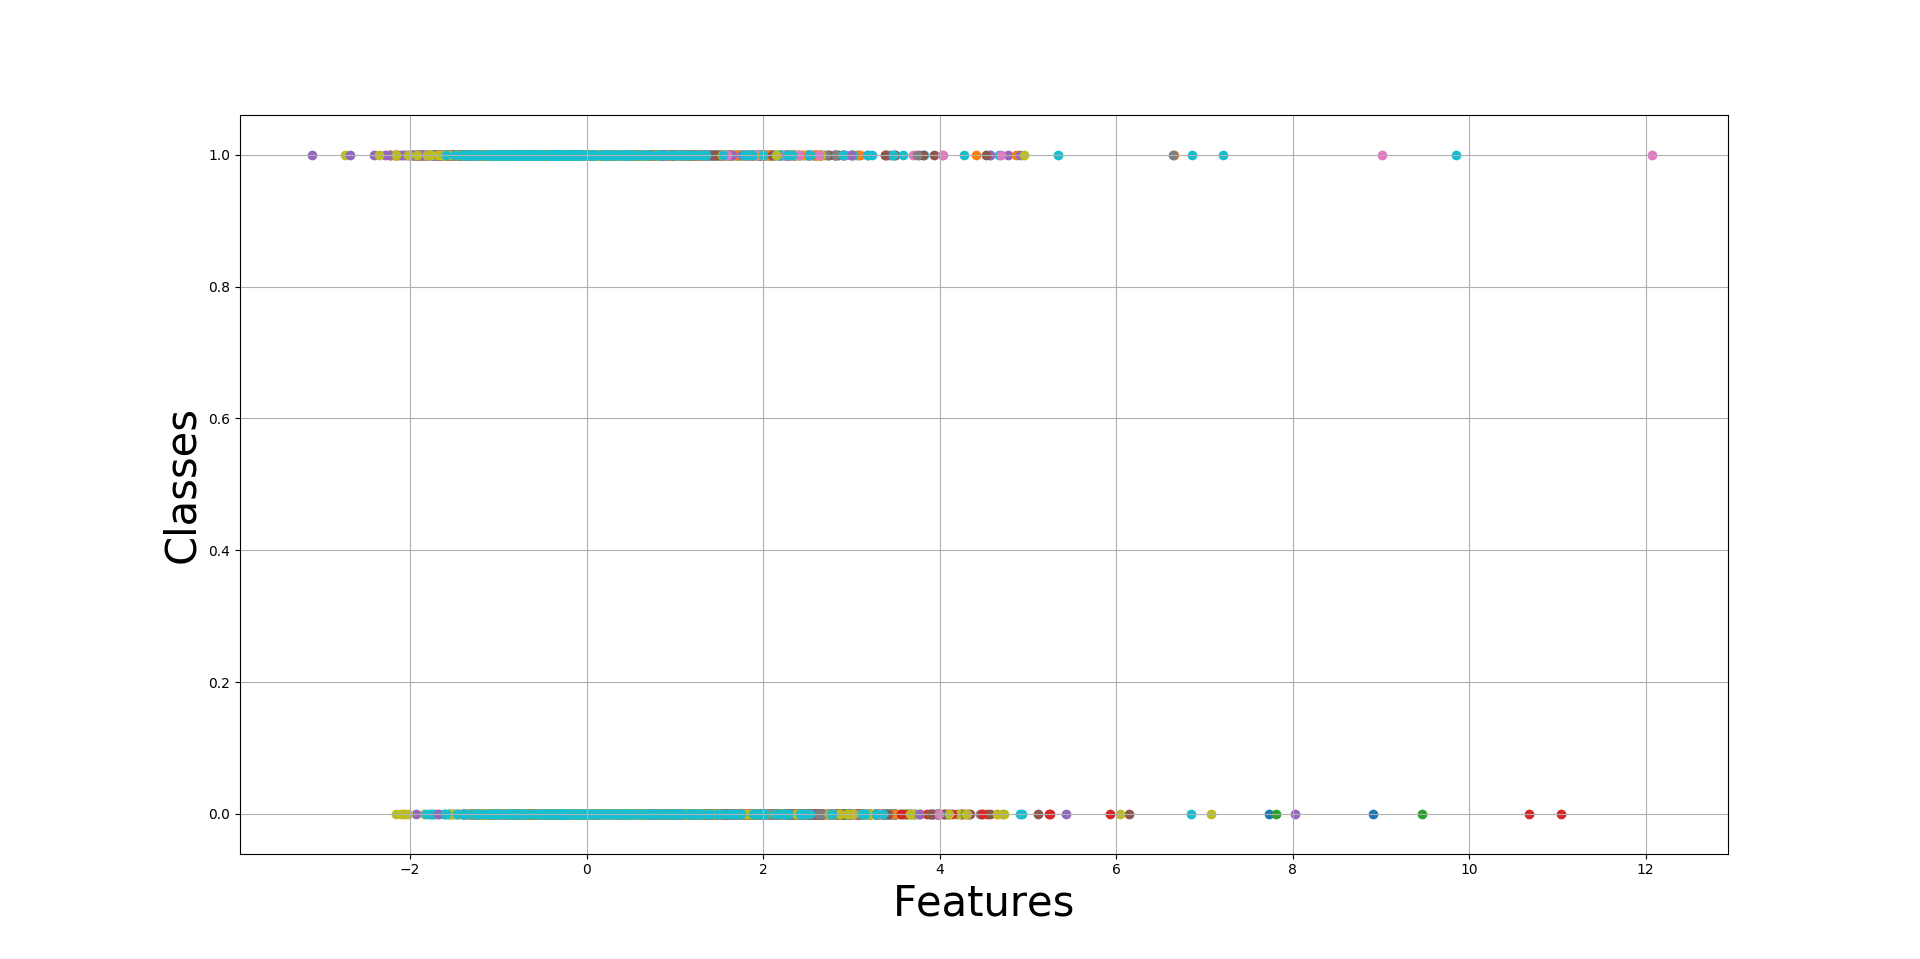
\includegraphics[width=\linewidth]{scatter_plot_data.png}
	\caption{Plotted using \texttt{matplotlib}\cite{Hunter:2007}. Scatter plot of the WDBC}
	\label{scatter-plot}
\endminipage\hfill
\end{figure}
\indent	Figure \ref{training-accuracy} shows the training accuracy of the ML algorithms: (1) GRU-SVM finished its training in 2 minutes and 54 seconds with an average training accuracy of 90.6857639\%, (2) Linear Regression finished its training in 35 seconds with an average training accuracy of 92.8906257\%, (3) MLP finished its training in 28 seconds with an average training accuraacy of 96.9286785\%, (4) Softmax Regression finished its training in 25 seconds with an average training accuracy of 97.366573\%, and (5) L2-SVM finished its training in 14 seconds with an average training accuracy of 97.734375\%. There was no recorded training accuracy for Nearest Neighbor search since it does not require any training, as the norm equations (Eq. \ref{taxicab-norm} and Eq. \ref{euclidean-norm}) are directly applied on the dataset to determine the ``nearest neighbor'' of a given data point $p_{i} \in \vec{p}$.\\
\indent	The empirical evidence presented in this section corroborates the findings of \cite{salama2012breast} and \cite{zafiropoulos2006support}, and attests to the effectiveness of ML algorithms on the diagnosis of breast cancer. While the experiment results are all commendable, the performance of the GRU-SVM model proposed in \cite{agarap2017neural} warrants a discussion. The mid-level performance of GRU-SVM with a test accuracy of 93.75\% is hypothetically attributed to the following information: (1) the non-linearities introduced by the GRU model\cite{Cho} through its gating mechanism (see Eq. \ref{z-gate} and Eq. \ref{r-gate}) to its output may be the cause of a difficulty in generalizing on a linearly-separable data such as the WDBC dataset, and (2) the sensitivity of RNNs to weight initialization\cite{alalshekmubarak2013novel}. Since the weights of the GRU-SVM model are assigned with arbitrary values, it will also prove limited capability of result reproducibility, even when using an identical configuration\cite{alalshekmubarak2013novel}.\\
\indent	Despite the given arguments, it does not necessarily revoke the fact that GRU-SVM is comparable with the presented ML algorithms, as what the results have shown. In addition, it was an expectation that the upper hand goes to the linear classifiers (Linear Regression and SVM) as the utilized dataset was linearly separable (see Figure \ref{scatter-plot}).

\section{Conclusion and Recommendation}

This paper presents an application of different machine learning algorithms, including the proposed GRU-SVM model in \cite{agarap2017neural}, for the diagnosis of breast cancer. All ML algorithms presented in Section \ref{ml-algorithms} exhibited high performance (all exceeded 90\% test accuracy) on the binary classification of breast cancer, i.e. determining whether benign tumor or malignant tumor. Consequently, the statistical measures on the classification problem were also satisfactory.\\
\indent	To further substantiate the results of this study, a CV technique such as $k$-fold cross validation should be implemented in the application of the specified ML algorithms. The application of such a technique would prove to be prolific as not only will it provide a more accurate measure of model prediction performance, but it will also assist in determining the most optimal hyper-parameters for the ML algorithms\cite{bengio2015deep}. Finally, dimensionality reduction techniques such as principal component analysis (PCA) may prove to be beneficial on the preprocessing of dataset, as evident from the findings of \cite{salama2012breast}.

\section{Acknowledgment}

An expression of gratitude to Dr. William H. Wolberg of the University of Wisconsin for the WDBC dataset used in this study. Also, an appreciation of the open source community, especially Cross Validated, GitHub, Google, Python, and Stack Overflow.